\section{Istruzioni per l'utilizzo}
\subsection{Requisiti hardware}
Non è richiesto nessun tipo di hardware particolare per il funzionamento dell'applicazione anche se è fortemento consigliato
l'utilizzo di una macchina non troppo vetusta.\\
L'unico requisito necessario è la possibilità di poter installare ed eseguire i principali browser in circolazione.\\
Al fine di un corretto funzionamento dell'applicazione è, inoltre, consigliata la fruzione da apparecchi Desktop e non Mobile sui quali non è
garantito il funzionamento corretto e ottimale.

\subsection{Requisiti software}
Per usufruire dell'applicazione SWEDesigner in ambiente Desktop sono consigliate le seguenti versioni dei seguenti browser:
\begin{itemize}
\item \emph{Google Chrome}, versione 49.x o superiore;
\item \emph{Mozilla Firefox}, versione 45.y o superiore;
\end{itemize}

\subsection{Prerequisiti}
Non sono necessari prerequesiti tecnici molto profondi per l'utilizzo dell'applicazione che non siano una conoscenza basilare dell'UML, del linguaggio Java e della Programmazionr ad Oggetti.
L'applicazione è comunque rivolta ad un pubblico di "tecnici" quindi non offre troppi aiuti nella costruzione dei diagrammi di classe e quelli per i metodi.

\subsection{Installazione}
Non è necessaria alcuna installazione dell'applicazione.

\subsection{Accesso all'applicazione}
Per accedere all'applicazione sarà sufficiente digitare all'interno del proprio browser l'URL fornito per l'accesso e, qualora non si fosse registrati al sistema, registrarsi con una e-mail, username e password.\\
Qualora si fossero perse le credenziali per l'accesso è possibile richiedere la password associata al proprio account per effettuare correttamente in login all'inerno del sistema.

\subsubsection{Registrazione}
Dalla pagina iniziale occorre cliccare su \textit{Registrati} e quindi inserire i propri dati all'interno dei campi dati. Terminato l'inserimento occorre premere il tasto \textit{Registrati}. In caso si desideri ritornare alla pagina iniziale basterà cliccare su \textit{Indietro}.\\
Non sarà possibile cliccare su \textit{Registrati} finché non saranno stati inseriti tutti i dati richiesti e al termine della registrazione verrà effettuata in automatico l'autenticazione.\\
\begin{figure}[H]
	\centering
		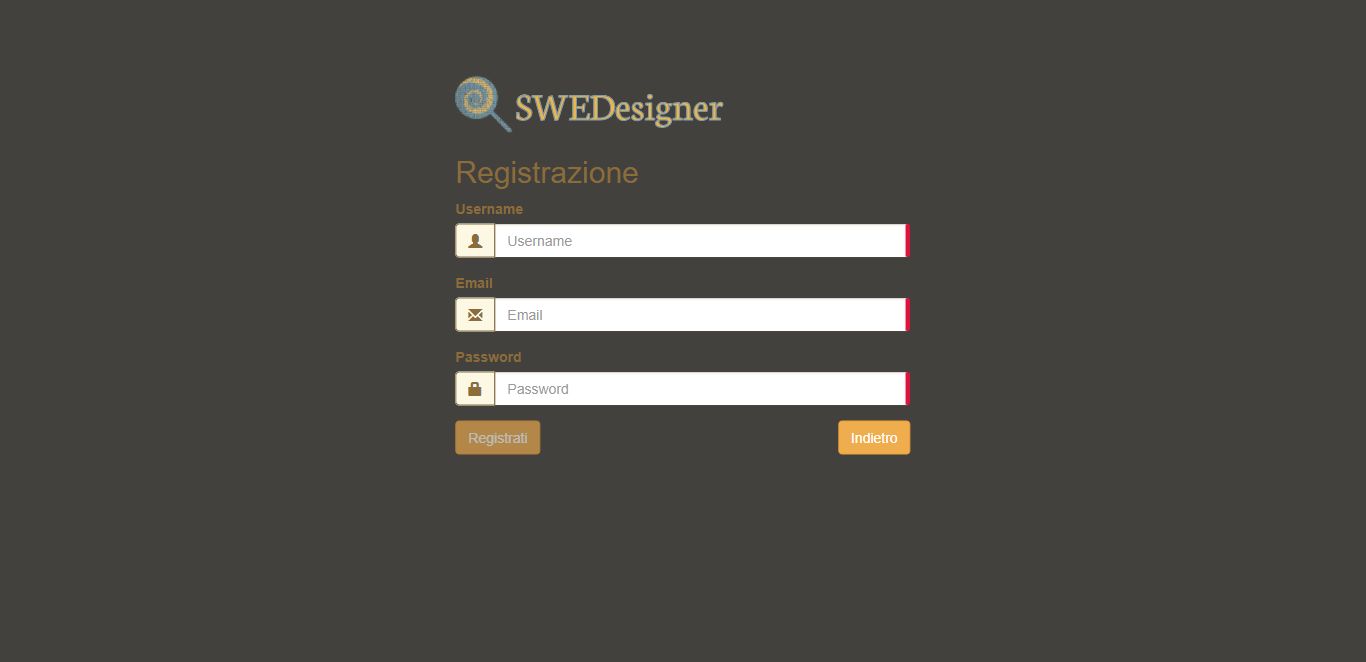
\includegraphics[width=1\linewidth]{res/img/registrazione.png}
	\caption{Pagina di registrazione}
\end{figure}
\newpage

\subsubsection{Autenticazione}
La pagina iniziale dell'applicazone corrisponde a quella di autenticazione all'interno della quale è necessario inserire le proprie credenziali per accedere al sistema.\\
Per effettuare l'autenticazione occorre inserire l'email e la password fornite durante la registrazione e poi cliccare su \textit{Login}.\\
All'interno di questa pagina è possibile recuperare la propria password mediante un click su \emph{Password dimenticata} oppure registrarsi mediante un click su \emph{Registrati}.\\
\begin{figure}[H]
	\centering
		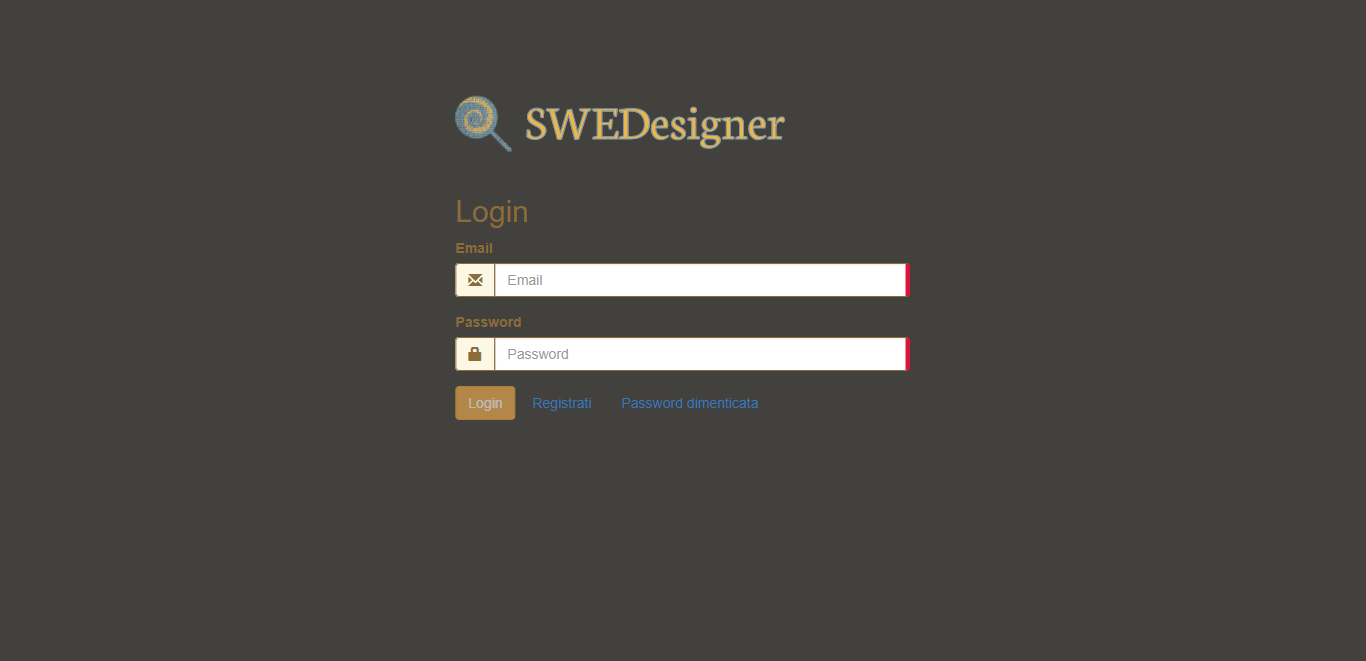
\includegraphics[width=1\linewidth]{res/img/autenticazione.png}
	\caption{Pagina iniziale}
\end{figure}
\newpage

\subsubsection{Recupero password}
Da questa pagina è possibile recuperare la propria password inserendo la propria e-mail all'interno dell'apposito campo dati e premendo il tasto \emph{Invia}.\\
Se si desidera ritornare alla pagina di autenticazione basterà cliccare su \textit{Indietro}.\\
Non sarà possibile cliccare su \textit{Invia} finché non sarà stata inserita la mail alla quale inviare la password.\\
\begin{figure}[H]
	\centering
		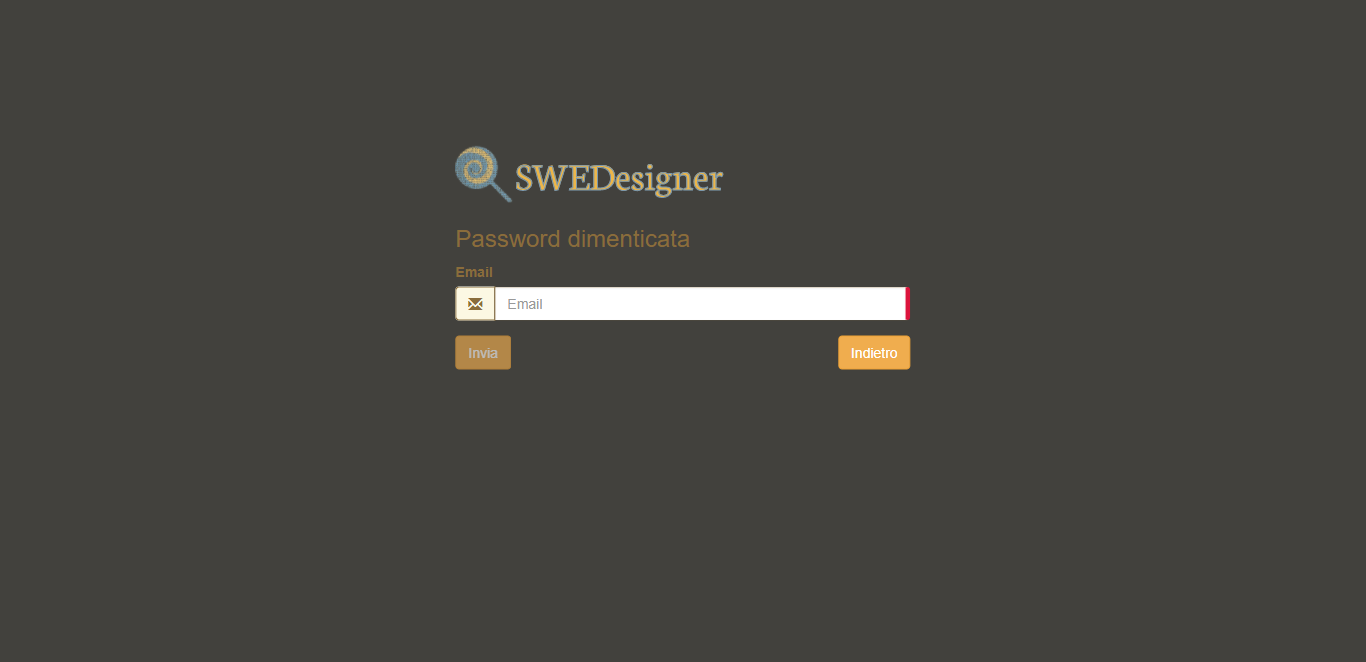
\includegraphics[width=1\linewidth]{res/img/password.png}
	\caption{Pagina di recupero password}
\end{figure}
\newpage
